\documentclass[../tp3_grupo404.tex]{subfiles}

\graphicspath{{\subfix{../out/}}}

\begin{document}

Para la solución al problema planteado se propone reducir el problema a un problema de corte de flujo
y solucionarlo con el algoritmo de Edmonds-Karp.

\begin{figure}[H]
    \centering
    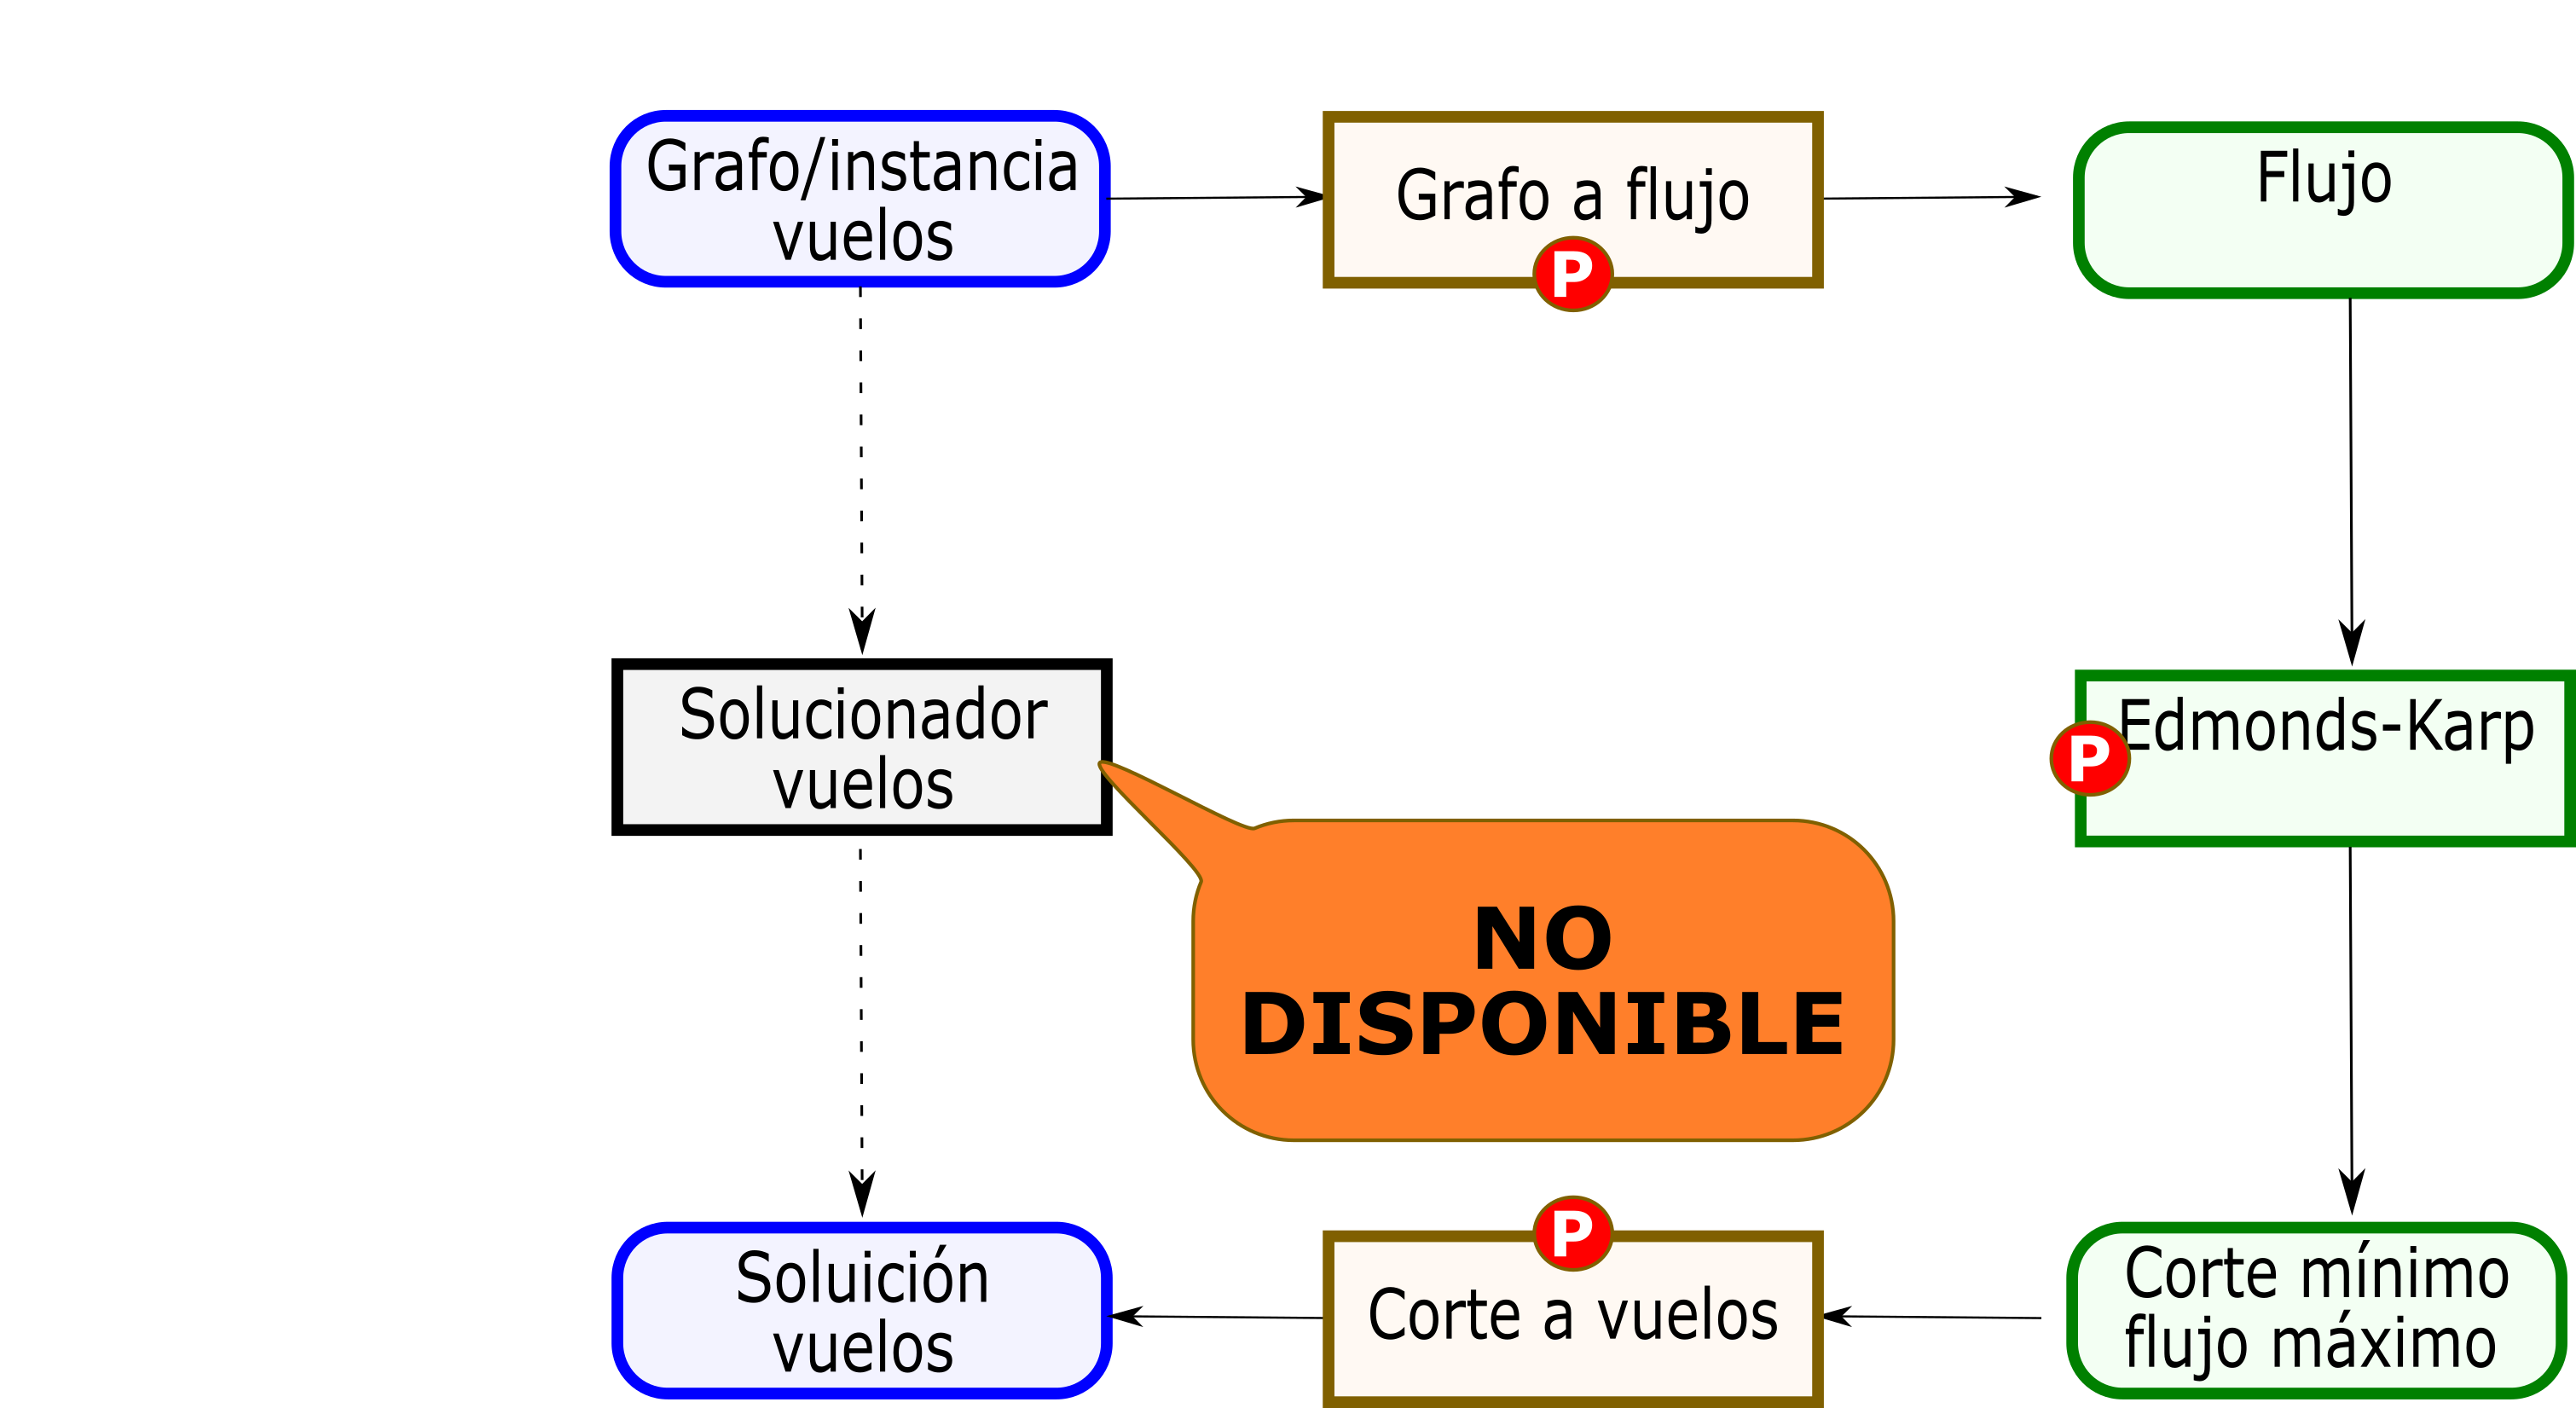
\includegraphics[width=0.9\linewidth,angle=0,origin=c]{out/reduc.png}
    \caption{\label{reduc}Reducción del problema, todas las operaciones son polinómicas.}
\end{figure}

En resumen, la solución completa sigue los siguientes pasos:
\begin{enumerate}
    \item Procesar el archivo en el formato dado a un grafo dirigido, utilizando lista de adyacencias.
    \begin{itemize}
        \item Cada nombre de aeropuerto es tratado como un número indicando la posición, en la lista
        de adyacencias, de cada lista de destino para un mismo origen.
        \item Cada elemento está compuesto por una tupla de id de destino y "peso" asociado.
        \item La estructura permite que peso pueda no ser simplemente un número, y el alias puede no ser un string.
            Pero en este punto, por el formato de entrada, sí lo serán.
    \end{itemize}
    \item Convertir el grafo en un diagrama de flujo, en el que:\begin{itemize}
        \item En cada arco original se almacena:\begin{itemize}
            \item una \textbf{capacidad máxima}, cuyo valor está dado por el anterior peso numérico del grafo.
            \item y un \textbf{flujo}, incialmente 0 (cero).
        \end{itemize}
        \item Cada arco original (a través de la clase \texttt{ArcoDirecto}) se obtiene un valor dado por
            la capacidad residual (la capacidad - el flujo). En el sentido contrario del grafo se almacena
            una referencia (a través de \texttt{ArcoInverso}) que, como valor, devuelve el flujo del arco
            directo (en el sentido original).
            \par Por ejemplo, un arco $A\underset{10}{\rightarrow}B$ es reemplazado por un ArcoDirecto
            $A\underset{0/10}{\rightarrow}B$ que devuelve un valor $10-0=0$, y se agrega un nuevo arco
            $B\rightarrow A$ (que referencia al anterior) y devuelve un valor igual al flujo ($0$).
    \end{itemize}
    \item Se aplica Edmonds-Karp: \begin{enumerate}
        \item Se inicializa en 0 un contador interno de flujo aumentado.
        \item Mientras haya un camino, encontrado con BFS, desde el origen y el destino dados en el archivo,
        cuyos arcos tengan valores mayores que cero:\footnote{Esto es, para un arco directo significa que
        hay un valor residual, el flujo no llegó a su capacidad máxima. para un arco inverso significa que
        hay un flujo en el sentido contrario que podría disminuirse.} \begin{enumerate}
            \item  Busca el cuello de botella (el menor de todos los valores).
            \item Aumenta el camino: Si es un arco directo, aumenta el flujo (reduciendo su "valor" y
            aumentando el del arco inverso asociado); si es un arco inverso, disminuye su flujo (aumentando
            su "valor", y reduciendo el del arco directo, ya que es el valor residual).
            \item Se aumenta un contador interno de flujo aumentado con el valor del cuello de botella.
        \end{enumerate}
    \end{enumerate}
    \item Al terminar, se recorre con un BFS todos los nodos a los que pueda llegarse por un arco no saturado,
        es decir donde no haya un valor directo de 0 (si lo hay se lo agrega aun subconjunto de arcos \texttt{corte}),
        y se los agrega al subconjunto A; el resto de los nodos pertenecen al subconjunto B.
    \item Se devuelve el contador de flujo como capacidad máxima de pasajeros del origen al destino,
    y el conjunto de arcos \texttt{corte} como los vuelos que cumplen con el criterio dado.
\end{enumerate}


% FIN DEL DOCUMENTO (SECCIÓN P1.1)
% NO BORRAR POR ACCIDENTE NI ESCRIBIR COSAS ABAJO
\end{document}